\documentclass[12pt]{article}

\usepackage{graphicx}

\begin{document}

\title{GrantSeer Documentation 1.0}
\author{Yang Song \\ yxs176@cse.psu.edu \\\\ Pennsylvania State University}
\date{}
\maketitle

\section{Introduction}
This document aims to guide you design reusable apps and loosely coupled system specifically based on new GrantSeer. GrantSeer originally developed by Dr. Puck Treeratpituk and written in Ruby on Rail. However, to improve the readability of the whole project and make it more maintainable, we decide to rewrite the system with Python and Django.

\subsubsection*{Who need to read this documentation}
\begin{enumerate}
	\item\ Anyone who wants to improve the current GrantSeer project.
	\item\ Anyone who wants to create new web apps that share the same database \texttt{csx\_exp}.
	\item\ Anyone who wants to know the very basic features about Django 1.6.
\end{enumerate}

\subsubsection*{Who shoud not read this documentation}
\begin{enumerate}
	\item\ Anyone who would like to know how to create a Django web app from zero.
	\item\ Anyone who works on a different database.
\end{enumerate}

The complete reference and tutorial of Django could be found at \\ https://docs.djangoproject.com/en/1.6/


\section{GrantSeer Architecture}
As we want to decouple the whole system, new GrantSeer is split into two services: \texttt{GrantSeerFrontendService} and \texttt{SeerBackendService}. In service design pattern, \texttt{Frontend Service} basically is responsible for interacting with users, generating request to \texttt{Backend Service} and rendering the data transferred from \texttt{Backend Service} for users. \texttt{Backend Service} is responsible for interacting with \texttt{MySQL} database, grouping and sorting those data and what not. In Django, \texttt{Backend Serivce} should be regarded as a data persistent layer of web app, even it could do more stuff.

\begin{figure}[!htb]
	\caption{GrantSeer Architecture}
	\label{grantseer_architecture}
	\centering
	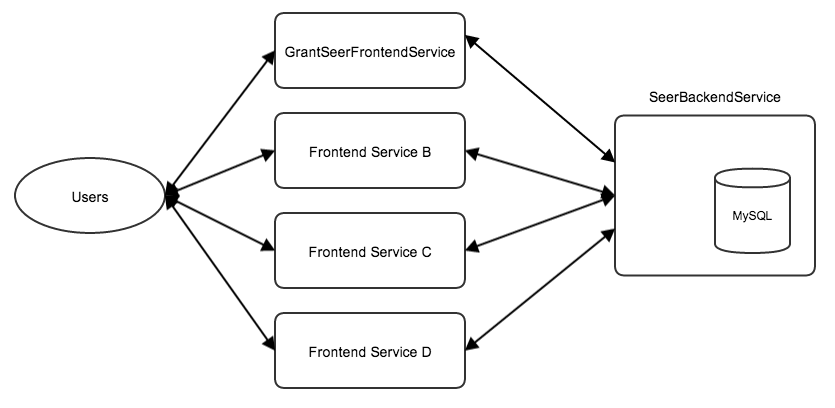
\includegraphics[width=\textwidth]{GrantSeerArchitecture.png}
\end{figure}

Figure \ref{grantseer_architecture} depicts architecture of GrantSeer. Currently only one frontend service exists. Developers are expected to add more frontend services that share the same database with \texttt{GrantSeer}. There are two reasons for this design.
\begin{enumerate}
	\item\ Distribute the workload. User requests only go to frontend services and different frontend services will handle different requests. \texttt{SeerBackendService} only handles requests that come from frontend services.
	\item\ Security. Only the ports that be able to reach frontend services are open. Malicious users are not be able to see \texttt{SeerBackendService}, so it's impossible to compromise backend service.
	\item\ Fail-safe. Even one or more frontend services are down, the rest of frontend services will be working normally.
\end{enumerate}

\section{Creating Frontend Service Project}
Your new frontend service should tightly-coupled with any other services in the current system, which means:
\begin{enumerate}
	\item\ Your frontend service should only send request to \texttt{SeerBackendService} and receive response from it.
	\item\ Your frontend service are NOT supposed to interact with other frontend services.
\end{enumerate}

Since your frontend service has to comply with these two rules, you have to create a new web apps from zero without filling database related configurations in the \texttt{settings.py} file.

Details about how to create a empty project and new app, please refer Django official documentation\footnote{https://docs.djangoproject.com/en/dev/intro/tutorial01/}, which will walk you through the basic things smoothly.

\section{Creating New App in SeerBackendSerivce}
This documentation will focus on some details about creating reusable apps in \texttt{SeerBackendService}. In this section, \texttt{SeerBackendService} folder always means folder \texttt{SeerBackendService/SeerBackendService}.

\subsection*{URL Mapping}
To make all apps in \texttt{SeerBackendService} maintainable, URL mapping plays significant role. In \texttt{SeerBackendService}, at least when we are designing this system, we create two \texttt{urls.py} files. One is under \texttt{GrantSeer} folder; another one is under \texttt{SeerBackendService} folder.

The \texttt{urls.py} file under \texttt{SeerBackendService} folder servers:
\begin{enumerate}
	\item\ Django admin pages
	\item\ index page. This page will take \texttt{HTTP GET} request and tells you if \texttt{SeerBackendService} is running or not.
	\item\ constructs urls for each apps. We will discuss it in the following paragraph.
\end{enumerate}

The \texttt{urls.py} file under \texttt{GrantSeer} folder only specifies its own urls that can be navigated to designated html pages. For example, \texttt{piname/\$} url will navigates to the method \texttt{GrantSeer.views.pi\_name}. But with the help of the \texttt{urls.py} under \texttt{SeerBackendService} folder, this url becomes \texttt{grantseer/piname/}. For each app, you should provide a index page that at least could provide information about the current status of the app.

In general, when you create a new app in \texttt{SeerBackendSerivce}, in \texttt{urls.py} under \texttt{SeerBackendService} folder, you should add a new url that includes all the urls of your new app. It is just like creating a namespace for each app so that you will not worry about duplicated urls when many people create new apps under the same project.

\subsection*{Models}
Django strictly follows MVC(Model-View-Controller) pattern. You will find a \texttt{models.py} file under \texttt{GrantSeer} folder. Basically, this auto-generated file wraps the underline database table and you are not supposed to change the content of this file unless the database structure has been modified.

Currently there is only one app in this project, so we still put \texttt{models.py} under \texttt{GrantSeer} folder. But if you want to create a new app and reuse this file, you strongly encourage you to move \texttt{models.py} to \texttt{SeerBackendService} folder as this will indicate that this file is supposed to share with other apps.

\subsection*{Data Wrapping}
When you splitting one component into two, data transferring is always on agenda. To the best of my knowledge, no consent about how your serialized data generated by backend service should be look like. In this project, we use JSON to wrap all the data.

When you look at \texttt{GrantSeer} web app source code, you may be curious about why we create may \texttt{DataWrapper} classes and \texttt{data\_wrapper} methods in \texttt{views.py} file.

The only reason is that the data generated by \texttt{SeerBackendService} contains lots of fields, including both attributes in database tables and other fields, such as number of pages, error messages, etc. For table attributes, Django provides a easy to to convert each rows you fetched from database to JSON. What you have to do is to call \texttt{serializers.serizlize('json', query\_result, fields=fields\_tuple)}. However, what you get from that is only the JSON data of your query results. To add more information to that data, we have to new \texttt{Data\_Wrapper} classes to hold those data and call \texttt{json.dumps(var(Custom\_Data\_Wrapper(\dots)))}. Then you are ready to send this JSON data back to frontend service.

However, if you could provide a more elegant way to wrap the data, please go ahead to modify the code and, if possible, to make everyone's life easier, provide APIs that everyone can call.

\end{document}
